\section{Planificación y presupuesto}
La siguiente sección detallará la organización y planificación del proyecto, 
junto con el presupuesto requerido para llevarlo a cabo, utilizando diagramas 
para facilitar la comprensión de los diferentes aspectos del proyecto.

\subsection{Plan de recursos humanos}
El éxito de cualquier proyecto se basa en la eficaz gestión y aprovechamiento 
de los recursos disponibles. Uno de los recursos más críticos y valiosos en 
cualquier proyecto es el equipo humano. En este plan de recursos, se describen 
los diferentes roles y responsabilidades de los integrantes del equipo, con el 
objetivo de garantizar una colaboración efectiva y la consecución de los objetivos 
del proyecto.

\begin{figure}[ht]
    \centering
    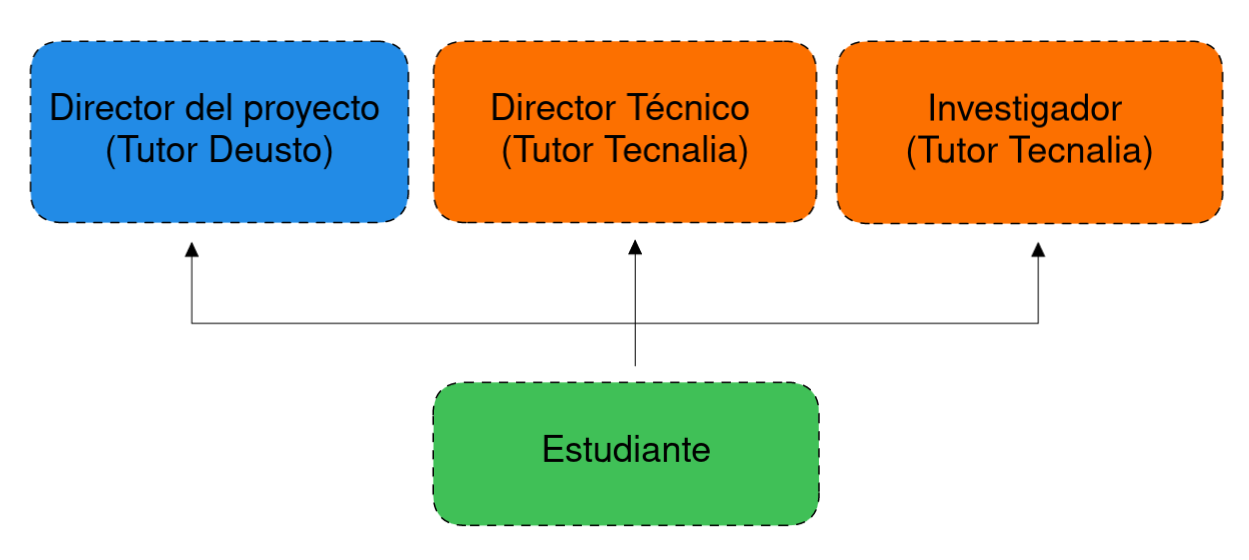
\includegraphics[width=\textwidth]{human-resources.png}
    \caption{Diagrama de recursos humanos}
    \label{fig:human-resources}
\end{figure}

\begin{itemize}
    \item \textbf{Director del proyecto:} El director del proyecto es la figura
    encargada de supervisar y coordinar todas las actividades del proyecto. Su papel 
    es fundamental para establecer una visión clara, comunicar los objetivos y metas, 
    y gestionar los recursos adecuados para alcanzarlos. Su experiencia en gestión de 
    proyectos, habilidades de liderazgo y capacidad para tomar decisiones son 
    fundamentales para asegurar la dirección correcta y el cumplimiento de los plazos 
    establecidos.
    \item \textbf{Director Técnico:} El Director Técnico desempeña un papel crucial 
    en la implementación exitosa del proyecto al proporcionar soporte técnico y 
    garantizar la calidad y el rendimiento del producto final. Su experiencia 
    técnica en el área específica del proyecto y su conocimiento profundo de las 
    herramientas y tecnologías pertinentes permiten tomar decisiones informadas 
    y resolver problemas técnicos de manera eficiente. Además, lidera y coordina al 
    equipo técnico, asegurando la correcta implementación de las soluciones propuestas.
    \item \textbf{Investigador:} El investigador supervisa y controla la calidad del 
    proyecto, identificando y proponiendo mejoras durante el proceso de desarrollo. Su 
    enfoque en el control de calidad asegura la entrega de un producto final de alto nivel.
    \item \textbf{Estudiante:} El estudiante es el encargado de llevar a cabo el proyecto,
    este constituye su TFG y asume la responsabilidad de llevar a cabo todas las fases del 
    mismo. Su participación abarca desde la investigación inicial hasta la implementación 
    y evaluación final del proyecto. Como investigador principal, realiza una investigación 
    exhaustiva sobre el tema del proyecto, recopilando información relevante y analizando 
    los enfoques existentes en el campo. Con base en esta investigación, define los objetivos 
    del proyecto y establece una estrategia para alcanzarlos.
\end{itemize}

\subsection{Programa de trabajo}
La siguiente sección detallará el programa de trabajo seguido en el proyecto, incluyendo 
las diferentes tareas realizadas con su duración planificada y real, junto con el diagrama 
de Gantt del proyecto. Las tareas del proyecto se han dividido en tres fases distintas. 
La primera fase incluye la formación necesarias para llevar a cabo el proyecto, así como
la investigación inicial y la definición de los objetivos. La segunda fase incluye la
implementación de las diferentes partes del proyecto, mientras que la tercera fase incluye
la evaluación y la documentación final.


\subsection{Presupuesto}
\subsubsection{Recursos humanos}
\subsubsection{Hardware}
\subsubsection{Software}
\subsubsection{Total}

\pagebreak